\begin{savequote}
  OR is the art of winning wars without actually fighting.
  \qauthor{Aurther Clarke}
\end{savequote}

\chapter{Introduction}

\section{Les origines de la recherche opérationnelle}
\label{sec:histoire}

\begin{wrapfigure}{i}{0.15\textwidth}
  \begin{center}
    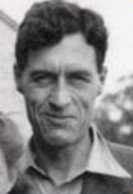
\includegraphics[width=0.14\textwidth]{Blackett-large.jpg}
  \end{center}
  \caption{Patrick Blackett}
\end{wrapfigure}

Les origines de la recherche opérationnelle, en abrégé RO, ne sont pas clairement définies, bien que Charles Babbage (1791--1871) soit souvent considéré comme le père de la recherche opérationnelle, en raison de ses travaux sur le coût du transport et le tri du courrier, menant à l'introduction du Penny Post en Angleterre, en 1840. %donner plus de détails.

Un siècle plus tard, la seconde guerre mondiale, de part son envergure, créa une besoin urgent d'allouer de manière efficace des ressources limitées aux différentes opérations militaires et aux activités au sein de chaque opération.
En particulier, l'organisation militaire britannique, puis américaine, mit à contribution un grand nombre de scientifiques pour gérer ces allocations, et s'occuper d'autres problèmes stratégiques et tactiques.
Ce faisant, ils furent appelés à poursuivre des recherches sur des opérations (militaires), et constituèrent les premières équipes de RO, notamment celle dirigée par Patrick Blackett, prix Nobel de physique en 1948~\cite{Kirb03}.
Leurs efforts furent significatifs dans la marche vers la victoire, par exemple en ce qui touche l'utilisation du radar, nouvellement développé.
Ces succès encouragèrent la poursuite de l'utilisation de la RO dans d'autres domaines.
La croissance importante de l'industrie d'après-guerre entraîna des problèmes, causés par la complexité croissante et la spécialisation dans les organisations, problèmes en fait proches de ceux présent lors du conflit.
Au début des années 1950's, la RO avait pénétré une multitude d'organisations commerciales, industrielles, et gouvernementales.
Et ce n'était que le début.

Au moins deux autres facteurs ont joué un rôle clé dans la croissance rapide de la RO.
Tout d'abord, des progrès substantiels ont été obtenus très tôt afin d'améliorer les techniques de RO.
Ces techniques, dans leur mise en pratique, furent soutenues par l'essor des outils informatiques.

\section{La nature de la recherche opérationnelle}
\label{sec:nature_ro}

``Rechercher sur des opérations'' touche tous les problèmes reliés à la conduite et à la coordination des opérations (activítés) au sein d'une organisation.
Cette organisation peut représenter des domaines très divers: l'industrie manufacturière, le transport, la construction, les télécommuncations, la finance, les soins de santé,\ldots.
La RO, associée à la révolution informatique, pénètre pratiquement tous les secteurs d'activités de la vie courante, même si sa présence est souvent invisible.

La première étape de la ``recherche'' est l'observation attentive du problème et sa formulation, ainsi que la collecte de données associées.
Il convient par la suite de construire un modéle scientifique qui tente l'abstraire l'essence du problème réel.
Tout modèle est une simplification de la réalité, mais cette représentation doit être suffisamment précise pour capturer les caractéristiques essentielles de la situation, et de pouvoir tirer des conclusions valides pour le problème réelle.
Il conviendra dès lors de tester ce modèle, et de le modifier au besoin.

Une caractéristique additionnelle est que la RO essaye souvent de trouver la meilleure solution (dite solution optimale) pour le problème examiné.
Cette solution peut ne pas être unique.
Cette recherche d'optimalité est un thème important en RO, même si son interprétation en terme managériels peut être délicate.
Il est difficile pour un individu de pouvoir maîtriser tous les aspects du problèmes à l'étude, de sorte que la RO est généralement plus un travail d'équipe, avec des experts en mathématiques, statistiques et probabilités, ingénierie, économie, administration, informatique, physiques, sciences comportementales, et les techniques spécifiques de la RO.

\section{Modélisation}
\label{sec:modeles}

Un modèle, telle que considéré dans ce cours, est une construction mathématique utilisée pour représenter certains aspects significatifs de problèmes du monde réel.
Il y a beaucoup de types différents de modèles mathématiques, mais nous nous focaliserons dans un premier temps sur les modèles d'optimisation.
Il y a trois composantes principales dans un modèle d'optimisation:
\begin{description}
\item[Variables:] elles représentent les composantes du modèle qui peuvent être modifiées pour créer des configurations différentes.
\item[Contraintes:] elles représentent les limitations sur les variables.
\item[Fonction objection]: cette fonction assigne une valeur à chaque configuration différente. Le terme ``objectif'' vient du fait que l'objectif est d'optimiser cette fonction.
\end{description}

\begin{example}[Un exemples de décisions binaires (oui/non)]
\label{sec:ex_villes}

Un étudiant en quête d'une université projette de visiter les campus de trois universités du Maine au cours d'un voyage unique, débutant et finissant à l'aéroport de Portland.
Les trois établissements sont dans les villes de Brunswick, Lewiston, et Waterville, et l'étudiant ne veut visiter chaque ville qu'une seule fois, tout en maintenant le trajet total le plus court possible.
Les distances entre ces villes sont données dans la Table~\ref{tab:distances}.

\begin{table}[htbp]
\begin{center}
\begin{tabular}{|c|c|c|c|c|}
\hline
Ville & Portland & Brunswick & Lewiston & Waterville \\
\hline
Portland & 0 & 26 & 34 & 78 \\
\hline
Brunswick & 26 & 0 & 18 & 52 \\
\hline
Lewiston & 34 & 18 & 0 & 51 \\
\hline
Waterville & 78 & 52 & 51 & 0 \\
\hline
\end{tabular}
\caption{Distances entre les villes (miles)}
\label{tab:distances}
\end{center}
\end{table}

L'étape la plus importante dans la construction d'un modèle est le choix des variables qui vont entrer en jeu.
Dans le présent cas, puisque n'importe quel trajet consiste en une série de petits déplacements entre deux villes, il est raisonnable d'assigner des variables aux décisions de partir ou non d'une ville vers une autre.
Pour plus de faciliter, numérotons les villes comme suit: 1 pour Portland, 2 pour Brunswick, 3 pour Lewiston et 4 pour Waterville. 
Ainsi, nous aurons une variable $x_{1,2}$ égale à 1 si l'étudiant voyage de Portland à Brunswick au cours de son parcours total, et 0 sinon.
Puisqu'il n'y a pas de voyage d'une ville vers cette même ville, nous avons d'ores et déjà les contraintes
\begin{equation}
x_{i,i} = 0,\ i = 1,\ldots,4.
\label{eq:dist_const_1}
\end{equation}
Une fois les variables choisies, nous pouvons essayer de formuler le problème.
Ce processus est en fait souvent une manière utile pour guider le choix des variables.

Chaque ville ne devant être visitée qu'une seule fois, elle ne peut apparaître qu'une seule fois comme ville d'arrivée.
En d'autres termes, pour $j$ fixé, $x_{i,j}$ ne peut être non-nul que pour un $i$ donné, avec $i \ne j$.
Une manière plus simple d'encoder cette information est d'écrire, pour $j = 1,\ldots,4$,
\[
x_{1,j} + x_{2,j} + x_{3,j} + x_{4,j} = 1,
\]
ou de manière plus concise.
\begin{equation}
\sum_{i = 1}^4 x_{i,j} = 1,\ j = 1,\ldots,4.
\label{eq:dist_const_2}
\end{equation}
Les contraintes formulées jusqu'à présent ne garantissent aucune forme de trajet ayant même départ et arrivée.
Par exemple, l'affectation $x_{1,2} = 1$, $x_{1,3} = 1$, $x_{1,4} = 1$, $x_{2,1} = 1$, et toutes les autres variables égales à 0, satisfont les contraintes~\ref{eq:dist_const_1} et \ref{eq:dist_const_2}.
Cette solution décrit toutefois un schéma de visites impossible puisque Portland est l'origine de tous les déplacements aux trois autres villes universitaires, mais n'est destination que depuis Brunswick.
Nous avons évidemment aussi besoin des contraintes
\begin{equation}
\sum_{j = 1}^4 x_{i,j} = 1,\ i = 1,\ldots,4,
\label{eq:dist_const_3}
\end{equation}
afin d'assurer que chaque ville ne serve d'origine que pour exactement un déplacement vers une autre ville.
Finalement, afin d'obtenir un véritable trajet ayant même origine et départ, nous devons rejeter les affectations qui décrivent des groupes déconnectés de petits déplacements comme $x_{1,2} = x_{2,1} = 1$, $x_{3,4} = x_{4,3} = 1$, avec toutes les autres variables égales à 0.
Nous pouvons forcer ceci avec les contraintes
\[
x_{i,j} + x_{j ,i} \leq 1,\ i = 1,\ldots, 4,\mbox{ et }j = 1,\ldots,4.
\]
Cette contrainte exclut tout mini-cycle.
%Exercise 1.1.2. Explain why we should not instead use the equation constraint xi, j +x j ,i = 1.

Les contraintes définies, nous devons décrire la distance totale associée à n'importe quel parcours autorisé.
Puisque nos variables ont seulement comme valeurs possibles 0 ou 1, nous pouvons multiplier chacune d'elle par la distance correspondante entre les deux villes indexées, et les additionner:
\[
\sum_{i = 1}^4 \sum_{j = 1}^4 x_{i,j} a_{i,j}.
\]
Notre modèle mathématique consiste à minimiser cette fonction, dite {\sl fonction objectif} par rapport aux variables $x_{i,j}$, tout en satisfaisant les contraintes préalablement décrites:
\begin{align*}
\min_x \ & \sum_{i = 1}^4 \sum_{j = 1}^4 x_{i,j} a_{i,j}, \\
\mbox{s.c.} \ & x_{i,i} = 0,\ i = 1,\ldots, 4, \\
& \sum_{i = 1}^4 x_{i,j} = 1,\ j = 1,\ldots,4, \\
& \sum_{j = 1}^4 x_{i,j} = 1,\ i = 1,\ldots,4, \\
& x_{i,j} + x_{j ,i} \leq 1,\ i = 1,\ldots, 4,\mbox{ et }j = 1,\ldots,4,\\
& x_{i,j} \in \lbrace 0, 1 \rbrace, \ i = 1,\ldots, 4,\mbox{ et }j = 1,\ldots,4.
\end{align*}
Ici, $x = (x_{i,j})_{i = 1,\ldots, 4, j = 1,\ldots,4}$, et {\sl s.c.}, ``sous les contraintes''.
Le problème d'optimisation ainsi construit constitue un {\sl programme mathématique}.

%\subsubsection{Résolution du programme mathématique}

Le problème de visites d'universités est assez petit que pour être résolu explicitement, sans recourir à des méthodes d'optimisation numérique.
Puisqu'il y a seulement trois parcours significativement différents, la distance totale associée à chacun d'eux pourrait être facilement calculée, et nous choisissons le parcours de longueur minimale, qui est ici
\begin{center}
Portland $\rightarrow$ Brunswick $\rightarrow$ Waterville $\rightarrow$ Lewiston $\rightarrow$ Portland.
\end{center}
avec une distance totale de 163 miles.
Il est cependant clair qu'une telle stratégie de résolution ne fonctionne plus comme le nombre de villes augmente.
\end{example}

\begin{example}[Un problème de mélange]

Un armateur doit construire un navire de guerre à partir de 50 tonnes d'acier contenant entre 0.5\% et 1.25\% de carbone (C), entre 0.3\% and 0.5\% de silicone (Si), pas plus de 0.05\% de sulfure (Su), et pas plus de 0.04\% de phosphore (Ph).
Un fournisseur produit de l'acier à partir de sept matières premières dont les qualités, les disponibilités en tonnes, et les coûts en \$/tonne sont donnés dans la Table~\ref{tab:steeldata}.
Le fournisseur veut déterminer la combinaison la moins coûteuse de composants bruts qu'il peut utiliser pour produire l'acier répondant aux besoins de l'armateur.
\begin{table}[htb]
\begin{center}
\begin{tabular}{lrrrrrr}
Matière première & \% C & \% Si & \% Su & \% Ph & Disponibilité & Coût \\
\hline
limonite & 3.0 & 0 & 0.013 & 0.015 & 40 & 200 \\
taconite & 2.5 & 0 & 0.008 & 0.001 & 30 & 250 \\
hématite & 0 & 0 & 0.011 & 0.05 & 60 & 150 \\
magnétite & 1.2 & 0 & 0.002 & 0.008 & 50 & 220 \\
silicone 1 & 0 & 90 & 0.004 & 0.002 & 20 & 300 \\
silicone 2 & 0 & 96 & 0.012 & 0.003 & 30 & 310 \\
charbon & 90 & 0 & 0.002 & 0.01 & 25 & 165 \\
\hline
\end{tabular}
\label{tab:steeldata}
\caption{Données pour le problème de production d'acier}
\end{center}
\end{table}

Puisque les fournisseur peut changer les quantités de matéries premières utilisées dans la producton de l'acier, nous pourrions assigner une variable différente pour représenter la quantiter de chaque matière première:
\begin{itemize}
\item
$x_1$ = tonnes de limonite,
\item
$x_2$ = tonnes de taconite,
\item
$x_3$ = tonnes d'hématite,
\item
$x_4$ = tonnes de magnétite,
\item
$x_5$ = tonnes de silicone 1,
\item
$x_6$ = tonnes de silicone 2,
\item
$x_7$ = tonnes de charbon.
\end{itemize}
Notons que les variables sont ici continues, contrairement à l'exemple précédent.

Afin de modéliser les contraintes, observons tout d'abord que
les variables dans ce cas sont naturellement bornées inférieurement par 0 (puisque des quantités négatives ne feraient pas de sens), et bornées supérieurement par leur quantité disponible, aussi avons-nous:
\begin{align*}
0 & \leq x_1 \leq 40, \\
0 & \leq x_2 \leq 30, \\
0 & \leq x_3 \leq 60, \\
0 & \leq x_4 \leq 50, \\
0 & \leq x_5 \leq 20, \\
0 & \leq x_6 \leq 30, \\
0 & \leq x_7 \leq 25.
\end{align*}
En supposant que n'importe quelle quantité d'une matière première contribue pour la même quantité d'acier, et en sachant que nous devons produire au moins 50 tonnes, nous avons
\[
\sum_{i = 1}^7 x_i \geq 50.
\]
Notons que nous ne supposons pas que nous produirons exactement 50 tonnes, puisqu'il peut être nécessaire de produire d'avantage afin de satisfaire les autres exigences du problème.

L'autre caractéristique contraignante dans ce problème que que l'acier doit contenir un certain pourcentage de carbone, de silicone, de sulfure et de phosphore.
Afin de voir comment ces exigences de composition se traduisent en contraintes par rapport à nos variables, nous nous concentrerons d'abord sur l'exigence d'avoir entre 0.5\% et 1.25\% de carbone, en espérant que les exigences sur le silicone, le sulfure et le phosphore se formulent de manière similaire.
À partir des données, nous connaissons le pourcentage de contribution en carbone de chaque matière première, aussi nous pouvons facilement calculer la quantité de carbone pour n'importe quel choix de variables comme
\[
0.03x_1+0.025x_2+0.012x_4+0.9x_7.
\]
Cependant, comme nous avons une exigences de proportion de carbone dans l'acier, nous devons diviser cette quantité de carbone par la quantité d'acier:
\[
\%C= 100 \left( \frac{\mbox{tonnes de carbone}}{\mbox{tonnes d'acier}} \right)
=
\frac{3.0 x_1+2.5 x_2+1.2 x_4+90 x_7}
{x_1+x_2+x_3+x_4+x_5+x_6+x_7}
.
\]
La contrainte que l'acier contienne entre 0.5\% et 1.25\% de carbone se traduit
dans la paire de contraintes
\begin{equation}
0.5 \leq
\frac{3.0 x_1+2.5 x_2+1.2 x_4+90 x_7}
{x_1+x_2+x_3+x_4+x_5+x_6+x_7}
\leq 1.25.
\label{eq:steel_composition}
\end{equation}
Les contraintes pour les autres composants se formulent de manière similaires.

Puisque ce problème implique de trouver la combinaison la moins coûteuse de matières premières qui rencontre la demande de 50 tonnes d'acier, la fonction objectif est simplement le coût des matières premières utilisées:
\[
\mbox{coût} = 200 x_1 + 250 x_2 + 150 x_3 + 220 x_4 + 300 x_5 + 310 x_6 + 165 x_7,
\]
où chaque matière première contribue pour son propre coût au total.
Le problème d'optimisation est dès lors la minimisation de cette fonction coût sur tous les choix des variables qui satisfont les contraintes modélisées.

Il n'est plus possible ici d'énumérer les solutions possibles afin de résoudre le modèle, en particuler puisque les variables considérées sont continues.
Nous pouvons néanmoins obtenir une intuition de la solution en considérant le comportement de la fonction objectif.
Ainsi, il est évident que celle-ci décroît quand une des variables diminue, et que la contribution la plus faible en termes de coût vient des variables avec les plus petits coefficients (i.e. les matières premières avec les coûts moindres par unité).
Si nous ignorons les contraintes de composition, le fournisseur devrait produire exactement 50 tonnes d'acier à partir des matières premières disponibles les moins chères.
Ceci signifierait utiliser 50 des 60 tonnes disponibles d'hématite (au coût de \$150 par tonne), pour un coût total des \$7,500.

Avant d'essayer de résoudre le problème d'optimisation complet (à l'aide d'un ordinateur), nous devrions réécrire les contraintes de composition dans une forme plus simple.
Par exemple, la contrainte \ref{eq:steel_composition} est nonlinéaire, mais peut être réexprimée comme deux contraintes linéaires en multipliant chaque terme des inégalités par le dénominateur.
Après la simplification de toutes les contraintes de composition de cette manière, et en utilisant un logiciel d'optimisation, nous obtenons la solution
\[
x_1 = 13.7888,\ x_3 = 35.8097,\ x_5 = 0.166667,\ x_7 = 0.234818,\ x_2 = x_4 = x_6 = 0,
\]
qui se traduit en exactement 50 tonnes d'acier, produit à partir de 13.7888 tonnes de limonite, 35.8097 tonnes d'hématite, 0.166667 tonnes de silicone 1 et 0.234818 tonnes de charbon.
Le coût total de production pour cette solution est \$8,217.96.
\end{example}


\section{Algorithmes et logiciels}

Au-delà de la modélisation, la résolution de problèmes de recherche opérationnelle nécessite de recourir à des algorithmes adapatés à la nature du problème, et capables de traiter de quelques dizaines à des millions de variables.
Leur étude consistera par conséquent une partie importante du présent document.
Même si de nombreux logiciels mettant en oeuvre ces algorithmes sont commerciaux, le monde de l'open-source n'est pas en reste avec notamment des projets tels que COIN-OR (\url{http://www.coin-or.org}). Il existe aussi diverses versions d'évaluations de solveurs commerciaux, ainsi que l'interface web NEOS (\url{http://www-neos.mcs.anl.gov}).
L'utilisation de tels outils nécessitent toutefois l'apprentissage de langages de modélisation adaptés; dans ce cours, nous nous baserons sur le langage GAMS (\url{http://www.gams.com}).
Ces langages servent à décrire dans des termes compréhensibles par le solveur le problème à résoudre.
La dernière version de IOR-Tutorial, développé en Java et proposé en complément à Hillier et Lieberman~\cite{HillLieb01}, peut également se révéler un complément précieux pour se familiariser avec les techniques de recherche opérationnelle.

\subsection{Un exemple avec GAMS}

GAMS est l'acronyme de General Algebric Modeling System.
Il consiste en un langage de description de problèmes, qui peut être compilé, et en une interface vers différent solveurs.
Une version gratuite de démonstration, permettant de résoudre des problèmes de petite taille, est disponible en téléchargement à l'adress \url{http://www.gams.com}.
Ce langage peut également être utilisé avec divers solveurs proposés sur NEOS.
Nous reviendrons plus en détail ultérieurement sur la formulation d'un programme mathématique avec GAMS, et nous contenterons d'un petit exemple introductif à ce stade.

Considérons un brasseur qui disposent des éléments suivants dans son stock:
\begin{enumerate}
\item
malt (75 kg);
\item
houblon (60 kg);
\item
levure (50 kg).
\end{enumerate}
Deux produits peuvent être obtenus: de la bière légère et de la bière noire.
Pour un kg de bière légère, il faut 2 kg de malt, 3 kg de houblon, et 2 kg de levure.
Pour un kg de bière noire, il faut 3 kg de malt, 1 kg de houblon, et 5/3 kg de levure.
La bière noire est vendue la moitié du prix de la bière légère.
En supposant que toute la production sera vendue, le brasseur souhaiterait décider des quantités de bières noire et légère à produire pour optimiser son profit.
Le programme GAMS résultant est
\begin{verbatim}
set b types of beer /light, dark/;

set i inputs /malt, hops, yeast/

parameter r(i) raw supplies /malt 75, hops 60, yeast 50/;

table a(i,b) input requirements

      light dark
malt  2     3
hops  3     1
yeast 2     1.67

parameter p(b) selling price / light 2, dark 1/;

variables pi profit (maximand)
          x(b) production level;

equations profit defines gross revenue
          supply(i) input supply constraint;

profit..     pi =e= sum(b, p(b) * x(b));
supply(i)..  sum(b, a(i,b)*x(b)) =L= r(i);

model beer /all/;

x.lo(b) = 0;

solve beer using lp maximizing pi;
\end{verbatim}

\begin{small}
\section{Notes}

Le contenu des Section~\ref{sec:histoire} et \ref{sec:nature_ro} se base principalement sur Hillier et Lieberman~\cite{HillLieb01}, Chapitre~1. La Section~\ref{sec:modeles} est construite à partir du Chapitre~1 de Levy~\cite{Levy09}. L'exemple GAMS est dû à Thomas F. Rutherford.

\end{small}
